\chapter{Introdução}\label{chp:LABEL_CHP_1}

\section{Motivação}\label{sec:LABEL_CHP_1_SEC_A}
Os processos de negócio consistem numa sequência de atividades e serviços que  encadeados cumprem determinado objetivo ou função na organização em que é desempenhado. A automatização de processos de negócio consiste na aplicação de tecnologia, de forma que uma ou mais atividades de um processo possam ser automatizadas, reduzindo assim a dependência de atuação humana para sua execução.\footnote{\url{http://www.lipsum.com/}}.

\section{Objetivos}\label{sec:LABEL_CHP_1_SEC_B}
O objetivo geral deste trabalho é propor uma solução para automatização de processos complexos que também conta com interação humana, inclusive durante o fluxo destes. Vamos apresentar uma ferramenta que permite a modelagem de fluxos variados, facilita a configuração e implementação, bem como a utilização contínua por usuários com conhecimentos básicos de processo e o acompanhamento deste por um gerente.

\section{Organização do texto}\label{sec:LABEL_CHP_1_SEC_C}

\chapter{Conceitos básicos}\label{chp:LABEL_CHP_2}

\section{Introdução}\label{sec:LABEL_CHP_2_SEC_A}

\section{Processos}\label{sec:LABEL_CHP_2_SEC_B}
Processo de negócio é um conjunto de atividades coordenadas, relacionadas entre si, que envolvem diferentes pessoas, procedimentos, áreas e tecnologias com o objetivo de gerar valor para a empresa, seja em forma de produtos ou serviços, internos ou externos.

\section{BPM}\label{sec:LABEL_CHP_2_SEC_C}
BPM é o acrônimo para o inglês Business Process Management, ou gestão de processos de negócio em português. Seu principal objetivo é oferecer uma abordagem sistemática para a execução, adaptação e melhoria de processos de negócio em um ambiente de constantes mudanças. O BPM pode ser encarado sob duas perspectivas distintas: o BPM como engenharia de software ou o BPM como disciplina de gestão.

\section{Activiti BPM}\label{sec:LABEL_CHP_2_SEC_D}


\section{Redmine}\label{sec:LABEL_CHP_2_SEC_E}
O Redmine é uma ferramenta de gerenciamento de projetos open-source. Foi criada por Jean-Philippe Lang em 2006. Desenvolvido em Ruby, utilizando a framework Rails, tem como objetivo dar flexibilidade de configuração ao usuário, e também ao desenvolvedor. A versão 3.1 deste software foi utilizada neste trabalho.


\chapter{Problema}\label{chp:LABEL_CHP_3}

\section{Introdução}\label{sec:LABEL_CHP_3_SEC_A}
Processos de negócio, quando realizados de forma desorganizada e despadronizada, levam à ineficiência organizacional. Neste capítulo, discutiremos uma alternativa para garantir que a execução das atividades das empresas sejam realizadas da maneira esperada e aumentar a capacidade de monitoramento de cada uma das etapas, que é a automatização de processos. 

\section{Automatização de processos}\label{sec:LABEL_CHP_3_SEC_B}


\chapter{Redmine}\label{chp:LABEL_CHP_3}

\section{Introdução}\label{sec:LABEL_CHP_3_SEC_A}
Neste capítulo vamos explicar como o Redmine, uma ferramenta de gerenciamento de projetos foi utilizada para gestão de processos, ilustrando com um exemplo. Vamos apresentar ainda, as capacidade extensiva desta ferramenta, através do desenvolvimento de plugins. Por último vamos abordar as limitações do Redmine, que nos motivaram a desenvolver algo novo para atingir nosso objetivo em automatização de processos.

\section{Gestão de processos com o Redmine}\label{sec:LABEL_CHP_3_SEC_B}


\section{Como automatizar um processo?}\label{sec:LABEL_CHP_3_SEC_C}

\section{Plugins}\label{sec:LABEL_CHP_3_SEC_D}
O Redmine foi desenvolvido de forma a ser extensível por meio de plugins. É possível modificar um funcionalidade da ferramenta, ou criar novas funcionalidades sem precisar alterar o código desta. Os plugins são desenvolvidos em Rails, a mesma linguagem de programação do Redmine. 

Para possibilitar extensões de funcionalidades que envolvem enxertar pedaços de código no meio de uma classe ou de uma tela, o Redmine disponibiliza hooks em diversas partes da ferramenta. São tags com um identificador da parte do código em que estão inseridas. E para utilizar este hook basta incluir um hook listener num plugin, e direcionar qual arquivo ou método um determinado hook vai disparar.

\section{Limitações}\label{sec:LABEL_CHP_3_SEC_E}


\chapter{Activiti BPM}\label{chp:LABEL_CHP_4}

\section{Introdução}\label{sec:LABEL_CHP_4_SEC_A}
Criado em 2010 por ex-integrantes do projeto jBPM, o Activiti BPM é um projeto de código aberto sob a licença Apache 2, que provê um motor BPM leve e completo sob a especificação BPMN 2.0. O Activiti é desenvolvido sob a linguagem de programação Java e é facilmente integrável com aplicações existentes por sua leveza e API amigável.

Neste capítulo vamos apresentar como o Activiti BPM pode ser utilizado na automatização de processos de negócio. Vamos apresentar ainda, a capacidade de modelagem de processos através da notação BPMN utilizada pelo Activiti. Por último vamos abordar as vantagens e limitações desta ferramenta frente às demais opções do mercado.

\section{BPMN}\label{sec:LABEL_CHP_4_SEC_B}
BPMN (Business Process Management Notation) foi criada para representar processos de negócio em forma de diagrama, através de uma notação padronizada e de fácil entendimento por diferentes profissionais, sejam desenvolvedores, analistas de negócio ou gestores. Foi criada inicialmente pelo BPMI (Business Process Management Initiative) em 2004, mas atualmente é mantida e atualizada pela OMG (Object Management Group). Sua versão mais atual é a BPMN 2.0, publicada em 2011.

Foi concebida sob a perspectiva de ajudar a cobrir a falta de entendimento entre diferentes departamentos e organizações a cerca de um determinado processo ou conjunto de processos, algo muito frequente no ambiente corporativo. Além disso, através de sua notação padronizada em XML (Extensible Markup Language), diferentes ferramentas podem fazer o uso de sua auto-descrição para orquestração de processos de negócio, sejam eles automatizáveis ou não.

A notação define quatro grupos distintos de objetos para permitir a diagramação de um fluxo de negócio. Os objetos são classificados em artefatos, agrupadores, conectores e objetos de fluxo. São utilizadas figuras geométricas, como retângulos e círculos, além de linhas pontilhadas e tracejadas, entre outros elementos para representar cada um dos objetos que constituem a notação.

1) http://searchcio.techtarget.com/definition/Business-Process-Modeling-Notation

2) http://blog.iprocess.com.br/2012/11/um-guia-para-iniciar-estudos-em-bpmn-i-atividades-e-sequencia

3) https://www.fluig.com/blog/entendendo-melhor-o-bpmn/

\begin{figure}
  \centering
  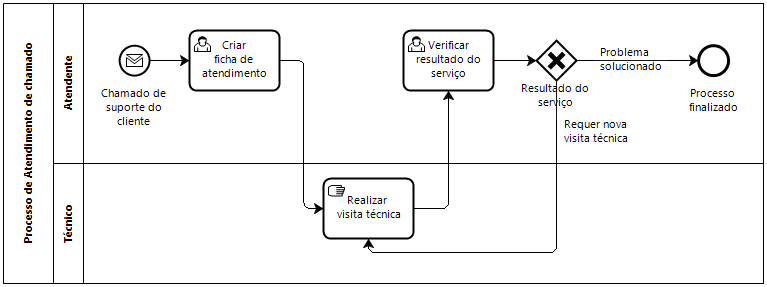
\includegraphics[width=1.0\textwidth]{imagens/bpmn_example.png}
  \caption{Exemplo de processo representado em BPMN}
  \label{fig:LABEL_FIG_1}
\end{figure}

\section{Gestão de processos com o Activiti BPM}\label{sec:LABEL_CHP_4_SEC_C}

\section{Como automatizar um processo?}\label{sec:LABEL_CHP_4_SEC_D}

\section{Vantagens e Limitações}\label{sec:LABEL_CHP_4_SEC_E}


\chapter{Integração Redmine e Activiti BPM}\label{chp:LABEL_CHP_5}

\section{Introdução}\label{sec:LABEL_CHP_5_SEC_A}
Dadas as vantagens e limitações das ferramentas Activiti e Redmine utilizadas como plataformas para a automatização de processos, decidimos desenvolver uma forma de integrá-las para explorarmos os pontos positivos de cada uma delas.

Para atingir este objetivo, criamos um plugin para o Redmine que possibilita a comunicação com o Activiti. Nas próximas sessões, descreveremos o processo de construção deste plugin e como utilizá-lo.


\section{Implementação}\label{sec:LABEL_CHP_5_SEC_A}

\section{Resultados}\label{sec:LABEL_CHP_5_SEC_A}